\chapter{Diseño e implementación de la solución.}
\epigraphhead [30]{%
  \epigraph{``Programar sin una arquitectura o diseño en mente es como explorar una gruta sólo con una linterna: no sabes dónde estás, dónde has estado ni hacia dónde vas.''}%
  {Danny Thorpe, programador.}%
}

En esté capítulo se describe cómo fue el diseño y comienzo del desarrollo del proyecto a partir de la idea redactada en los capítulos anteriores. 

\section{Punto de encuentro de ambos proyectos paralelos.}
	El punto de encuentro acordado entre ambos proyectos para su posterior unión se fijó en el interfaz donde el estado de la adquisición es controlado y los datos adquiridos pueden ser obtenidos. Se especificó el siguiente diseño del interfaz para que ambas partes se desarrollen en torno al mismo:

	\subsection{Especificación del interfaz de control de adquisición de datos piDA.}\label{subsec:especificacion_piDA}
	\begin{itemize}
		\item[•] \_\_init\_\_(): Constructor de la clase para gestionar una adquisición con los parámetros por defecto (Frecuencia de muestreo 0 -la máxima posible-, canal de entrada 0, máximo número de muestras 0, sin límite).
		\item[•] \_\_init\_\_(sampling rate): Constructor de la clase para gestionar una adquisición a la frecuencia de muestreo que se pasa como argumento. Una frecuencia de muestreo 0 no fuerza ningún tiempo de espera entre muestras consecutivas, con lo que las muestras se toman a la mayor tasa posible. El resto de parámetros toman sus valores por defecto.
		\item[•] \_\_init\_\_(sampling rate, channel): Constructor de la clase para gestionar una adquisición a la frecuencia de muestreo y del canal de entrada dados con el número máximo de muestras por defecto.
		\item[•] \_\_init\_\_(sampling rate, channel, max count): Constructor de la clase para gestionar una adquisición a la frecuencia de muestreo, del canal de entrada y con el máximo número de muestras a adquirir (0 si no hay límite) dados.
		\item[•] set\_sampling\_rate(sampling rate): fija la frecuencia de muestreo de la adquisición. Una frecuencia de muestreo 0 no fuerza ningún tiempo de espera entre muestras consecutivas, con lo que las muestras se toman a la mayor tasa posible.
		\item[•] get\_sampling\_rate(): devuelve la frecuencia de muestreo que se ha fijado para la adquisición.
		\item[•] set\_channel(channel): fija el canal de entrada del que se toman las muestras.
		\item[•] get\_channel(): devuelve el canal de entrada que se ha fijado para la adquisición.
		\item[•] set\_max\_count(max count): fija el número máximo de muestras que se pueden tomar. 0 no fija ningún límite.
		\item[•] get\_max\_count(): devuelve el número máximo de muestras fijado para la adquisición.
		\item[•] start(): comienza la adquisición.
		\item[•] stop(): detiene la adquisición.
		\item[•] get\_data(): devuelve una lista con todos los datos adquiridos hasta ese instante. Cada miembro de esa lista es a su vez una lista de dos elementos: el primero es el tiempo de adquisición (.\emph{float}) y el segundo el valor de la adquisición (\emph{int}).
		\item[•] get\_data(n\_count): devuelve una lista con los últimos n\_count datos adquiridos.
		\item[•] get\_status(): devuelve el estado en el que se encuentra la adquisición: ’waiting’, ’running’, ’stopped’.
		\item[•] get\_elapsed\_time(): devuelve la duración del periodo de ejecución de la adquisición.
		\item[•] print\_data(): escribe en pantalla un listado de todos los datos adquiridos hasta ese instante. 
		\item[•] print\_data(n\_count): escribe en pantalla un listado de los últimos n\_count datos adquiridos.
	\end{itemize}

\section{Primeras fases del desarrollo.}	
\subsection{Creando el sistema base.}
	Dado que la solución a desarrollar no se trata solo del software, sino de un equipo informático completo similar a un ordenador personal, lo primero que se ha investigado es cómo combinar el SBC con los distintos periféricos -teclado, ratón, pantalla- para conformar el producto final.
	
	El teclado y el ratón ha sido lo más sencillo de elegir, ya que la única exigencia es que sean USB para poder ser enchufados a la Raspberry Pi y su coste es muy reducido (menos de 10€ ambos periféricos).
	
	No ha sido el caso de la pantalla: La Raspberry Pi dispone de dos tipos de salida de vídeo: el estándar digital relativamente nuevo HDMI capaz de una resolución de hasta 1080p\footnote{1920x1080 píxeles proyectados progresivamente (un fotograma cada vez)}, y el modo analógico totalmente obsoleto Composite (mediante un conector RCA, como las antiguas conexiones de los DVDs o videoconsolas a los televisores de tubo) capaz de una resolución máxima de 576i\footnote{576 \emph{líneas} entrelazadas, se muestra la mitad de la imagen cada vez proyectando las líneas pares o impares alternamente.}) 
	
Esto dota a la Raspberry Pi de cierta flexibilidad al contemplar un estándar compatible con prácticamente todos los televisores del mercado en los últimos 30 años y también disfrutar de una calidad de vídeo digital acorde con los tiempos con HDMI, pero el interés se centra en poder conectar el SBC a los monitores disponibles en los laboratorios y despachos de la Facultad. Actualmente la práctica totalidad de los monitores disponibles para los alumnos en la facultad funcionan bajo el estándar VGA, no HDMI. Se investigó la posibilidad de convertir ese HDMI digital en VGA analógico. Una vez conseguido un viejo monitor Dell de 17'' se probaron diferentes adaptadores y convertidores económicos.
	
		Una de las comunidades en internet sobre la Raspberry Pi mantiene una \emph{Wiki}  donde se han comparado ya distintos adaptadores y cables\cite{VerifiedPeripherals_vga}. Se eligieron de la lista dos modelos de coste contenido (menos de 6€) y comentarios positivos.
Desgraciadamente uno de los mismos no funcionó como se esperaba (solo 640x480 de resolución en la pantalla, muy insuficiente para una aplicación actual) pero el otro adaptador (\autoref{fig:hdmi-to-vga}) en cambio funcionó a la perfección, adaptándose automáticamente a la pantalla a la que fuera conectado. En el caso del monitor Dell del que se dispone: 1024x768, en otras pruebas se alcanzaron 1280x1024 y según especificaciones del producto, podrían obtenerse resoluciones de hasta 1920x1080. 

\begin{figure}[!Hb]
\centering
  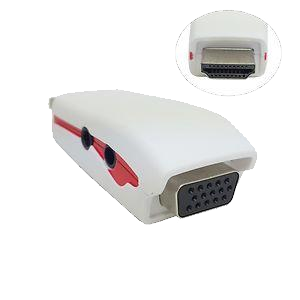
\includegraphics[width=0.40\textwidth]{img/hdmi-to-vga-output-projector-monitors-adapter.png}
  \caption{Adaptador HDMI a VGA.}	\label{fig:hdmi-to-vga}
\end{figure}


\pagebreak
Con esto ya se dispone de un equipo completo y funcional. El desglose de elementos y su precio es el siguiente:

\begin{savenotes}
\begin{table}[!ht]
  \centering
  \begin{tabular}{| c | c | c | c | c | c |}
  	\hline
    Elemento & Cantidad & Precio \\ \hline
   Raspberry Pi Model B & 1 & \pounds{24,35} (30,50€) \\ \hline
   Tarjeta de memoria SD de 4GB clase 10\cite{amazon_SD4GB} & 1 & 5,90€ \\ \hline
   Adaptador HDMI-VGA\cite{dhgate_vga} & 1 & \$7,82 (5,85€) \\ \hline
   Teclado USB\cite{amazon_tecladousb} & 1 & 6,99€ \\ \hline
   Ratón USB\cite{amazon_ratonusb} & 1 & 4,90€ \\ \hline
   Cargador de móvil 5v 700mAh\cite{amazon_cargadorusb} & 1 & 7,49€\footnote{Aunque los hay más económicos, en este aspecto se prefiere calidad ante precio ya que muchos de los disponibles en el mercado a precios económicos resultan no ofrecer el rendimiento esperado, y en un dispositivo como la Raspberry Pi induce al malfuncionamiento o la avería de la misma.} \\ \hline 
  \end{tabular}
  \caption{Desglose de coste de la solución propuesta.}
  \label{tab:desglose_precios}
\end{table}
\end{savenotes}

El total asciende a 54,14€, un precio muy atractivo comparado con lo que cuesta cualquier ordenador personal hoy en día. El precio no incluye el coste del monitor, puesto que se reciclaría alguno de los existentes en el centro. De no ser así, el precio ascendería unos 70€ por un modelo estándar y se seguiría requiriendo el adaptador HDMI-VGA, puesto que el coste de un monitor VGA sigue siendo aún inferior al de uno digital con HDMI.

Estos son los requerimientos técnicos y económicos para el sistema base en el que correrá el software que se ha desarrollado en este proyecto. Esto no incluye los elementos electrónicos y hardware necesarios para poder adquirir datos de los sensores, ese es el propósito del proyecto paralelo, ejecutado bajo las mismas premisas que éste.


\subsection{Eligiendo el entorno de desarrollo.}
	Es básico antes de comenzar el desarrollo de una aplicación informática elegir un entorno donde realizar la programación del mismo, para ello existen los IDEs (entornos de desarrollo) y Python dispone de gran cantidad de ellos\cite{wikipython_ide}: desde entornos ya conocidos a estas alturas como Netbeans hasta grandes productos corporativos como son Visual Studio o XCode. Un IDE permite simplificar la tarea del desarrollador al proveer herramientas como depuradores, sintaxis de colores para su mejor lectura, compiladores integrados, etc. Además algunos incluyen su propio constructor de interfaces gráficas (\emph{GUI builder}) con el que la tarea de diseño se hace intuitivamente y de forma visual en lugar de tener que ``dibujarla'' escribiendo con el teclado.
	
	Sin embargo, se ha preferido prescindir de un IDE propiamente dicho por dos razones en concreto:
\begin{enumerate}
	\item Se carece de la experiencia en Python necesaria para realizar un proyecto de estas dimensiones, por tanto para realizar un aprendizaje sólido en el mismo la mejor solución es programar todo a mano y encontrarse con los problemas que todo novato ha de encontrarse.
	\item Por norma general, \emph{programar} un interfaz gráfico a través de una herramienta gráfica suele ser irónicamente más costoso que escribiéndolo a mano y conociendo las herramientas disponibles para la ordenación de los elementos, así como creando esquemas en bolígrafo y papel de qué se quiere crear. 
\end{enumerate}

Por estas razones, se ha decidido utilizar el editor de texto \emph{Sublime Text 2} para el desarrollo de todo el proyecto. Además, con respecto al segundo punto y el código innecesario añadido por los constructores de interfaces gráficos, ha resultado mucho más práctico saber en todo momento qué es lo que está computando el procesador en cuanto a la GUI, pues la Raspberry Pi es conocida por ralentizarse a la hora de procesar gráficos.

\subsection{Eligiendo el framework gráfico.}
	\emph{Python} dispone de múltiples frameworks gráficos\cite{wikipython_guiprogramming} libres para elegir en el desarrollo de nuestra aplicación. En total se ha probado con dos posibilidades multiplataforma: Tkinter y WxPython.

\subsubsection{Tkinter.}
	Este framework tiene como punto a favor que está integrado de serie con Python y evita al programa de depender de librerías externas. Además la programación en Tkinter\cite{effbot_introductiontkinter} resulta muy sencilla puesto que no hay una cantidad exagerada de controles o \emph{widgets}\footnote{Cada uno de los elementos con los que un interfaz gráfico interactúa con el usuario: botón, caja de texto, menú, etc.} ni muchas opciones de personalizar los mismos.
	
	 No obstante, ésta es la misma razón por la que se desiste su uso: tras probar diversas implementaciones de lo que podría ser la solución final se descubrió que es una librería poco potente y más orientada a realizar pequeños diálogos o ventanas que a realizar un programa relativamente grande con multitud de controles.
	
\subsubsection{WxPython.}
		\emph{WxPython} es una versión para Python del famoso \emph{WxWidgets}\cite{wxwidgets} en C++ con toda la versatilidad y calidad de su predecesor. Ésta ha sido la librería elegida para nuestro programa ya que su API, aunque esté pobremente documentada\cite{wxpython_apifea} y muchas veces directamente copiada de la versión en C++, ha resultado suficientemente potente.		
		
		No obstante, en otras versiones\cite{wxpython_apiphoenix} de la documentación, ésta es más explícita, está escrita para Python e incluso muestra la apariencia de los widgets en las distintas plataformas.
		
	En su contra además se puede añadir que es un framework que requiere de más \emph{artesanía} pero cuyos resultados saltan a la vista rápidamente y necesita ser instalado aparte. Este no es un problema realmente ya que el gestor de paquetes \emph{Aptitude} (más conocido por su comando \emph{apt-get}) de nuestro sistema operativo \emph{Raspbian} lo dispone en sus repositorios oficiales y su instalación se ha automatizado en un script que acompaña al código del programa.
	
\subsection{Eligiendo una librería de representación gráfica.}
	Una de las funciones fundamentales de la aplicación será mostrar los datos adquiridos mediante una gráfica con respecto al tiempo, por tanto se necesita una librería que permita realizarlo o por otra parte programar una librería propia adaptada al uso. La \emph{wiki} de Python\cite{wikipython_plotting} ofrece muchas alternativas. La primera de ellas y elegida en este proyecto es Matplotlib, compatible con el framework gráfico WxPython (o \emph{WxWindows}).
	
	Matplotlib dispone en su página web\cite{matplotlib_home} de multitud de ejemplos (\autoref{fig:matplotlib_examples}) de todo lo que es capaz de hacer y llama la atención que integra la posibilidad de exportar los datos dibujados en multitud de formatos como PNG, PDF o SVG así como su potente herramienta de zoom. Además dispone de un extenso API con todas las posibilidades que ofrece.
	
	Otra alternativa que podría haberse elegido podría haber sido Plotly, pero su uso requiere de registro en su página web y conexión a internet para verificar el mismo cada vez que se utilice. Esto resulta muy molesto e innecesario, especialmente si se desea que esta solución se implemente en varias estaciones de trabajo y se desconoce si dispondrán conexión a internet. Como alternativa \emph{más libre} está Veusz, pero no resulta especialmente atractivo visualmente.
	
\begin{figure}[hb]
  \centering
  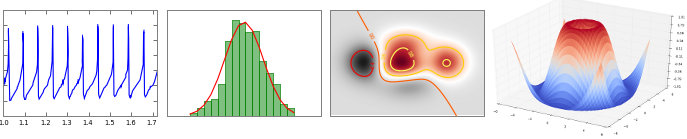
\includegraphics[width=1\textwidth]{img/matplotlib-caps.png}
  \caption{Ejemplos de Matplotlib.}\label{fig:matplotlib_examples}
\end{figure}
\section{Consideraciones a tener en cuenta antes de comenzar.}

\subsection{Dos soluciones muy distintas.}
	Las dos interfaces que se pretenden sustituir con este proyecto son muy diferentes entre sí: si bien ambas usan gráficas o histogramas para la representación de los datos, la mecánica interna de cómo obtener los datos y procesarlos es muy distinta. Por acuerdo mutuo se decidió realizar primero la solución que se ve más simple tanto a nivel electrónico como a nivel de procesado: la del laboratorio de termodinámica y física aplicada y su dispositivo \emph{PASCO 500 Interface}.
	
	Es el más sencillo porque la adquisición de datos no necesita tanta frecuencia de muestreo\footnote{Velocidad a la que se obtienen los datos.} y se pueden procesar fácilmente. En cambio para el laboratorio de radiactividad se necesitarían varios miles de hercios, algo que se ve muy inviable para hacer directamente en la Raspberry Pi sin la necesidad de un hardware externo complejo con el que no se ha contado durante el desarrollo de este proyecto. 
	
\subsection{El método de trabajo a utilizar.}
	Solo hay un único desarrollador, por lo que ha habido flexibilidad total a la hora de elegir el método de trabajo. En este caso se ha efectuado el desarrollo mediante pequeños hitos diarios desarrollando cada parte del programa. Como se ha utilizado Git como repositorio de software, se ha adoptado la norma de que todo lo que se envíe al repositorio ha de funcionar. Por tanto al llegar a cada hito se ha procedido a testar el programa contra fallos, se han corregido los más críticos y documentado los más leves en cada envío al repositorio. Por tanto el cumplimiento del método ha sido estricto al no poder dejar un objetivo a medias, que dejaría el programa no utilizable o parcialmente inutilizable.
	
	Al haber ofrecido el grupo un despacho donde trabajar a ambos proyectos paralelos, la comunicación ha sido bidireccional y regular, proponiendo cambios y comentando la implementación de las diversas partes diariamente. Además durante gran parte del desarrollo se han realizado reuniones semanales en una sala de juntas con los codirectores de ambos proyectos y los proyectandos en orden de clarificar dudas, preguntar alternativas de desarrollo o consejos en general.

